\chapter{Projekt systemu}
\label{cha:analizaAplikacji}

\section{Architektura systemu}
\label{sec:architektura}
Architetura aplikacji jest typowa dla frameworku Ruby on Rails. Żądania od klienta są kierowane do serwera aplikacyjnego. Serwer kieruje żądania użytkowników do dyspozytora który przekierowuje żądanie do odpowiedniego kontrolera. Kontroler korzystając z mechanizmu ActiveRecord, który jest odpowiedzialny za mapowanie obiektów z bazą danych, otrzymuje konkretne dane. Następnie kontroler może przekierować żądanie oraz dane do innego kontrolera lub wysłać odpowiedź do użytkownika poprzez wyrenderowanie odpowiedzi w przeglądarce klienta lub poprzez moduł ActionMailer, który jest odpowiedzialny za wysyłanie wiadomości mailowych. Zadania które mają się wykonywać w tle trafiają do modułu ActiveJob, który jest odpowiedzialny za odpowiednie zakolejkowanie zadań i wywołanie ich w odpowiednim czasie.
\noindent
\begin{minipage}{\linewidth}
\makebox[\linewidth]{
  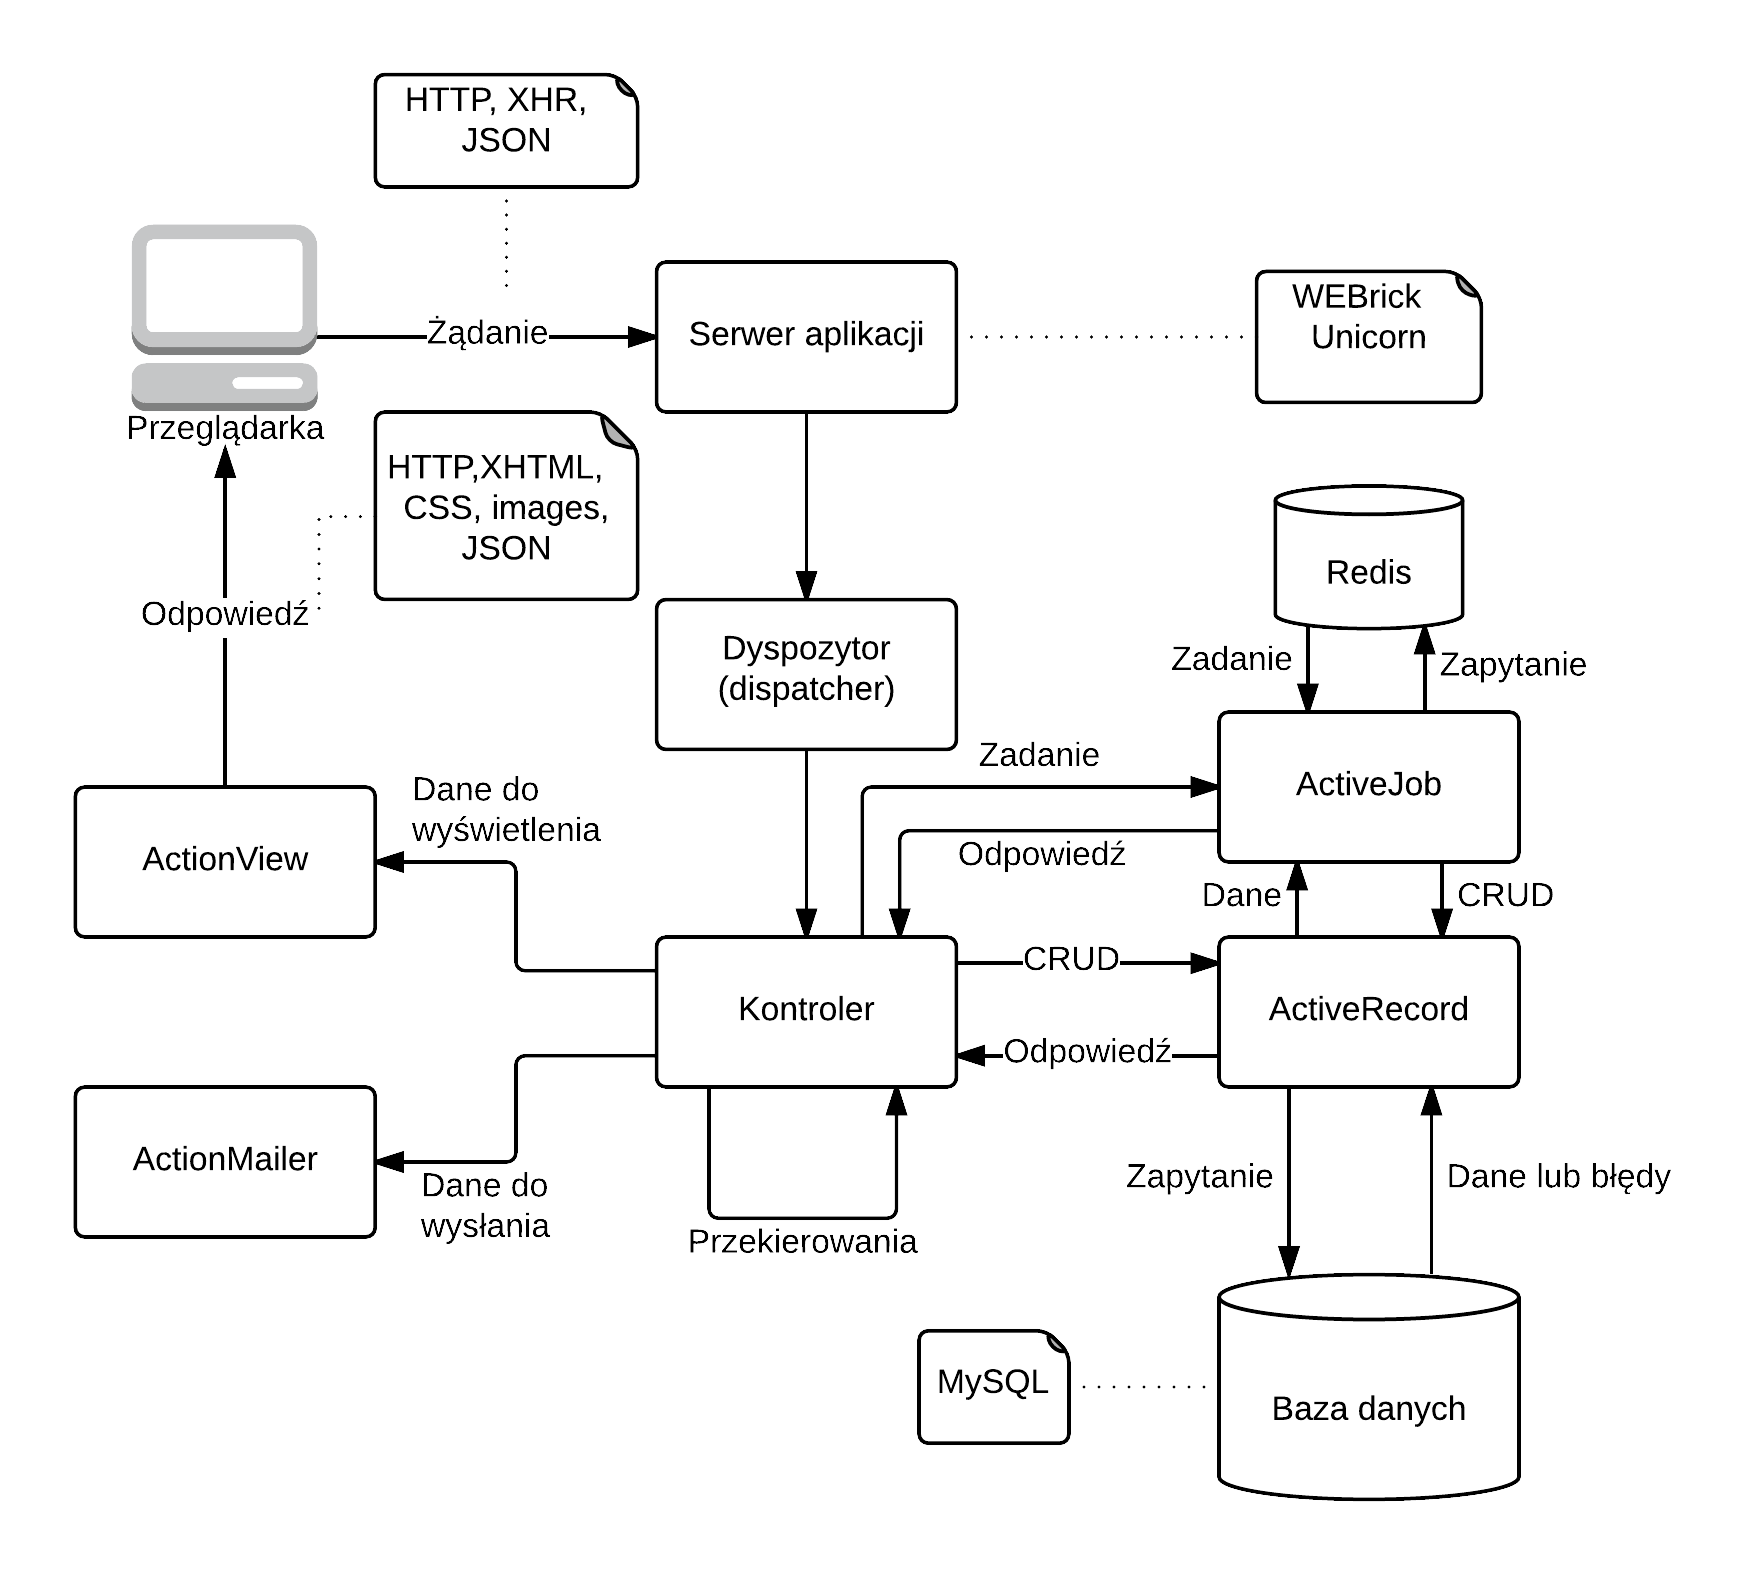
\includegraphics[keepaspectratio=true,scale=0.8]{pictures/architecture.png}}
\captionof{figure}{Diagram architektury}\label{use-case}
\end{minipage}

\section{Model bazy danych}
\label{sec;modelBazyDanych}
\noindent
\begin{minipage}{\linewidth}
\makebox[\linewidth]{
  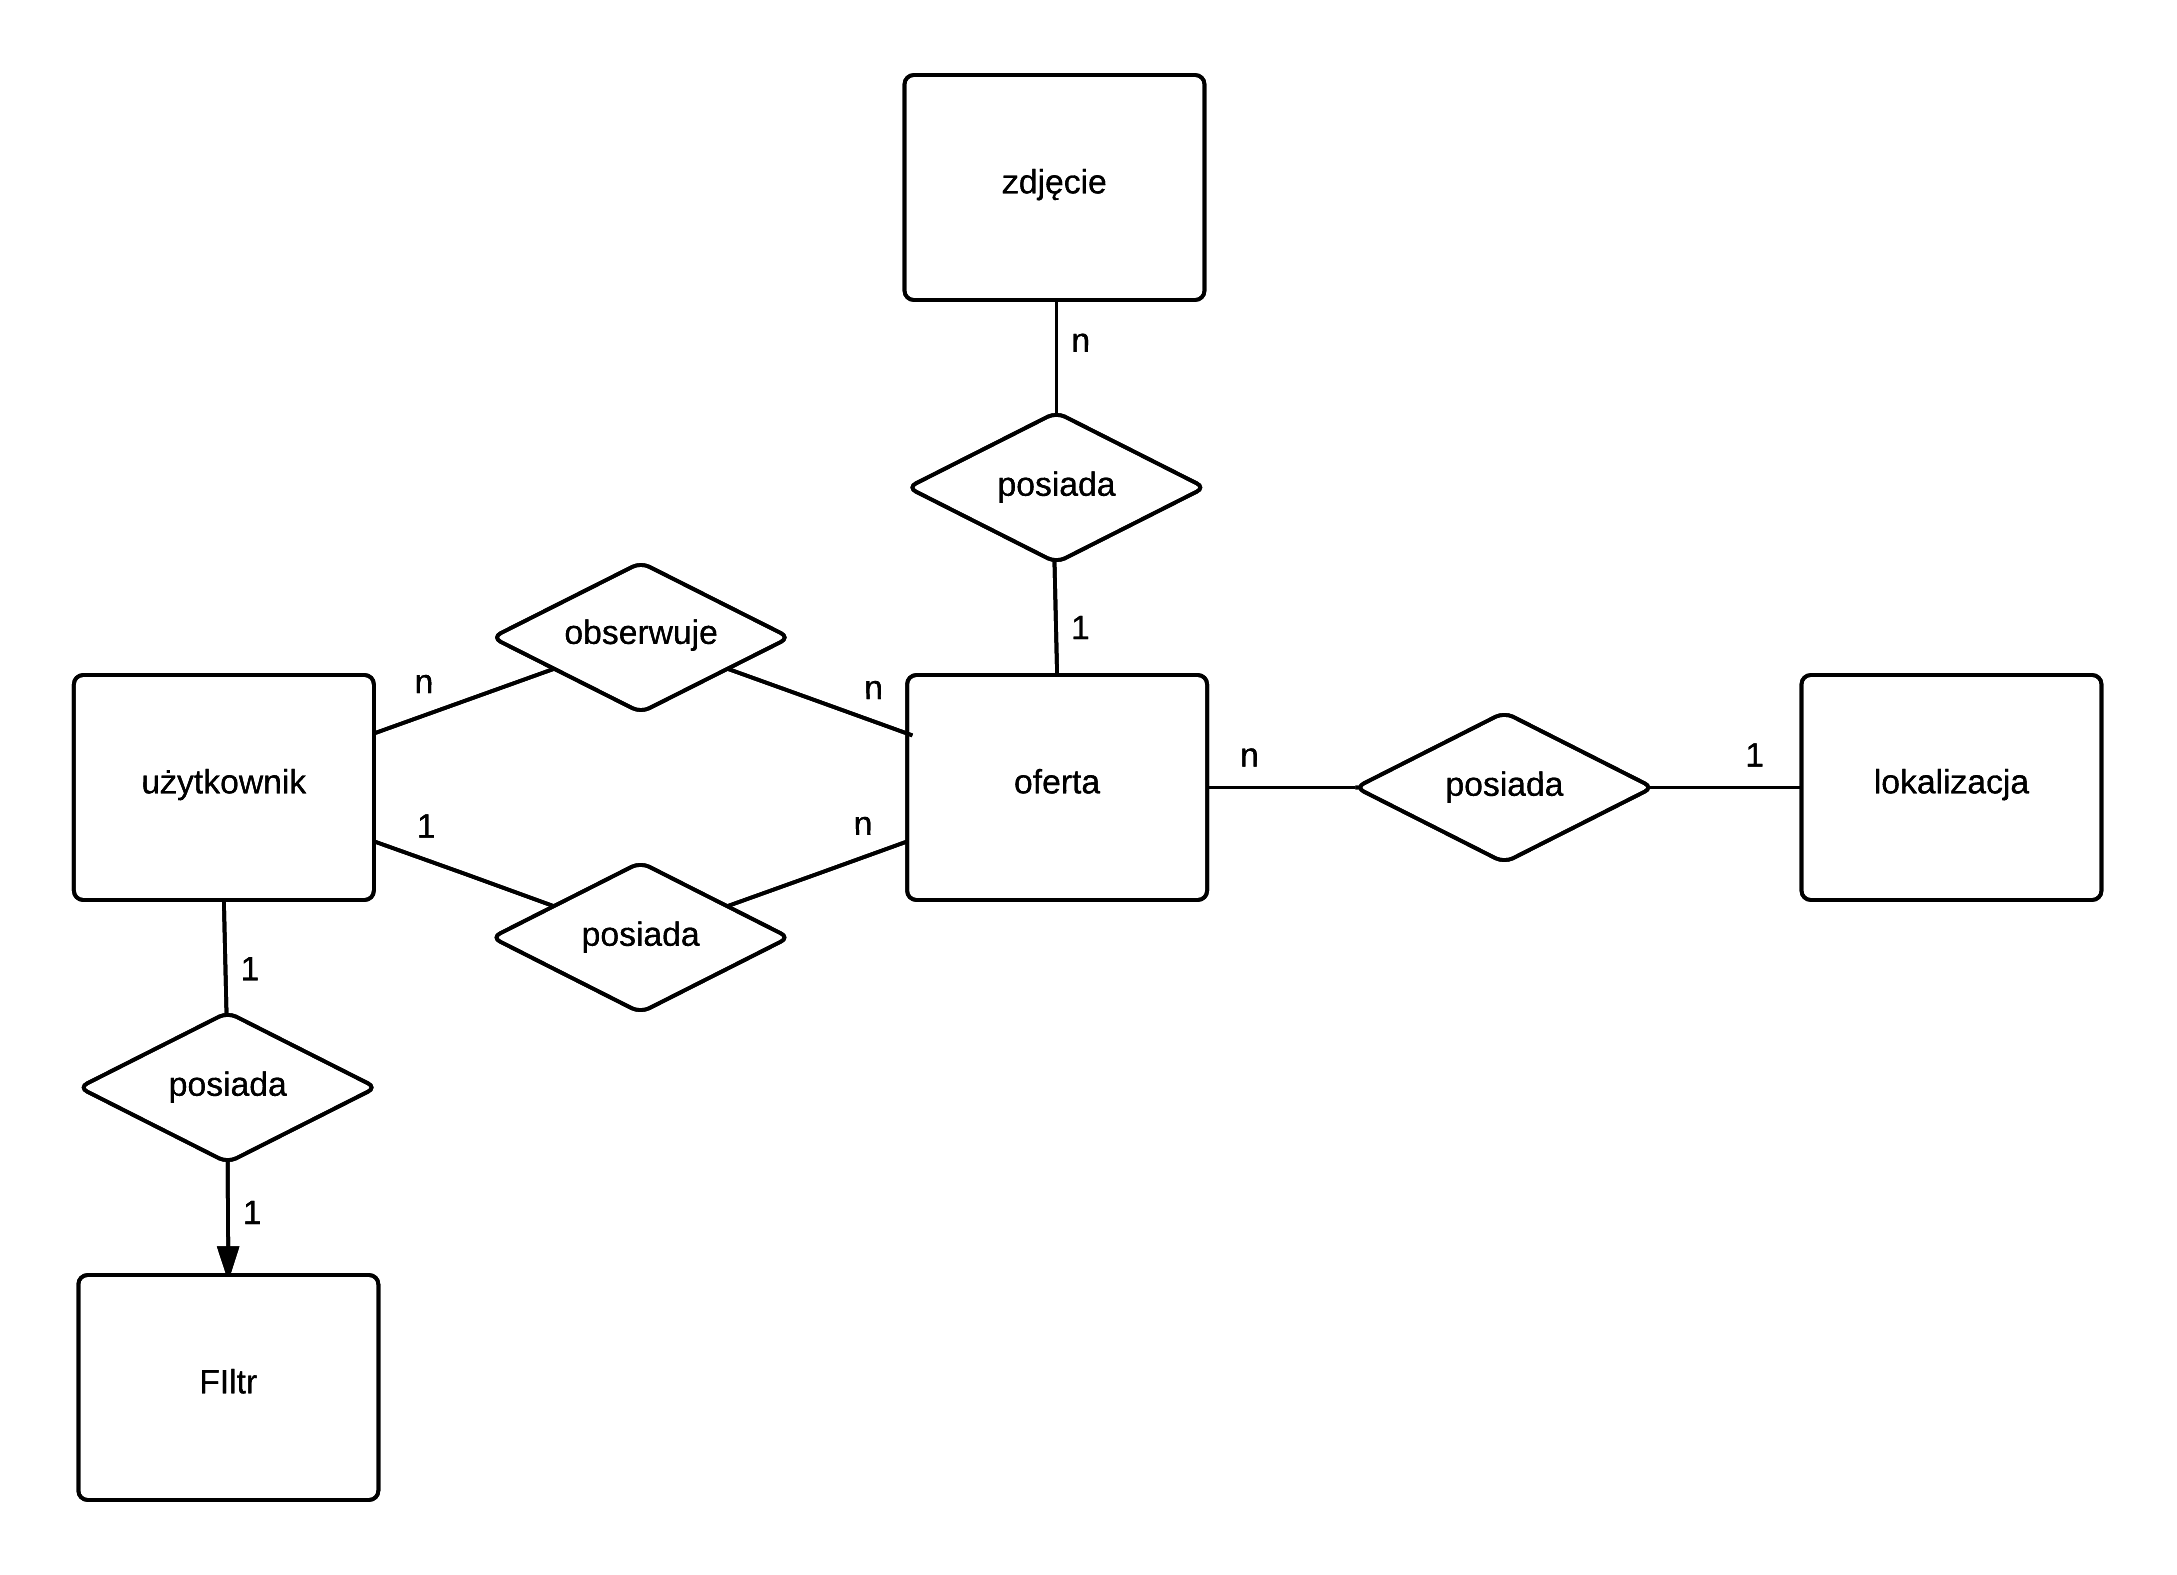
\includegraphics[keepaspectratio=true,scale=0.9]{pictures/erd.png}}
\captionof{figure}{Diagram ERD bazy danych}
\end{minipage}

\section{Interfejs graficzny}
\label{sec:interfejsGraficzny}
Strona graficzna aplikacji jest utrzymana w konwencji charakterystycznej dla aplikacji typu Single Page Application. Konwencja ta polega na umieszczeniu całej aplikacji oraz wszystkich funkcjonalności na jednej stronie interentowej w celu wywołania u użytkownika odczucia płynnego działania aplikacji podobnego do zwykłych aplikacji komputerowych. W technice tej cały potrzebny kod aplikacji (kod HTML, arkusze stylów CSS, skrypty JavaScript) jest pobierany podczas pierwszego załadowania aplikacji. Potrzebne elementy są dołączane dynamicznie do już załadowanej strony zazwyczaj jako odpowiedź na wywowałanie akcji przez użytkownika. Techniką która umożliwia dynamiczne generowanie treści strony jest dzięki bibliotece JavaScript jQury. Biblioteka ta umożliwa wykorzystanie XMLHttpRequest ze skryptów JavaScript. Żądania i odpowiedzi mogą być przesyłane bez konieczności przeładowywania strony. Każde wywołanie akcji przez użytkownika skutkuje wyświetleniem dodatkowego okna na stronie umożliwiającym wykonanie akcji, np. logowania, rejestracji.(Flanagan, David, "JavaScript - The Definitive Guide", 5th ed., O'Reilly, Sebastopol, CA, 2006, p.497)

Zazwyczaj oferty w serwisach ogłoszeniowych są wyświetlane jako lista. Jest to dosyć niewygodne podejście gdyż, użytkownik nie może zbyt szybko ocenić czy dane ogłoszenie jest dla niego interesujące. W opisywanej aplikacji zdecydowano się na zaimplementowanie zupełnie odmiennego sposobu prezentacji ofert. Ofety są prezentowane jako znaczniki na mapie dzięki czemu, każde ogłoszenie jest nierozerwalnie związane z lokalizacją. Zarówno znaczniki jak i mapa pochodzą z Google Maps API. W celu filtrowania dostępnych ofert aplikacja dostarcza zestaw filtrów, którymi użytkownik może swobodnie manipulować. 

\section{Interfejs restowy}
\label{sec:interfejsRestowy}

\section{Opis struktury danych oferty}
\label{sec:strukturaOferty}
Kluczową strukturą dla poprawnego działania całego programu jest struktura oferty. Jest to bardzo rozbudowany model, lecz było to konieczne ze względu na dużą liczbę atrubutów którymi oferty muszą być opisane. Atrybuty oferty można podzielić ze względu na typ:
\begin{itemize}
\item Numeryczny całkowity
\begin{itemize}
\item size - rozmiar mieszkania w metrach kwadratowych
\item rooms - liczba pokoi
\item people - liczba osób mogących mieszkać w danej lokalizacji
\item floor - piętro budynko
\item views - liczba wyświetleń oferty
\end{itemize}
\item Znakowy
\begin{itemize}
\item offer\_type - typ oferty
\begin{itemize}
\item O - od właściciela
\item A - od agencji mieszkaniowej
\end{itemize}
\item location\_type - typ lokalizacji 
\begin{itemize}
\item H - dom
\item F - mieszkanie
\item R - pokój
\end{itemize}
\item building\_type - typ budynku
\begin{itemize}
\item H - dom
\item T - kamienica
\item A - blok
\end{itemize}
\item parking\_type - typ parkingu
\begin{itemize}
\item N - brak możliwości zaparkowania auta
\item R - istnieje możliwość ale miejsce nie jest gwarantowane
\item O - miejsce gwarantowane niezadaszone
\item G - miejsce w garażu
\end{itemize} 
\item heating\_type - typ ogrzewania
\begin{itemize}
\item G - gazowe
\item E - elektryczne
\item C - Centralne - opał stały
\item D - ogrzewanie miejskie
\end{itemize}
\end{itemize}
\item Numeryczny niecałkowity
\begin{itemize}
\item parking\_price - cena za parking
\item media\_price - opłata za wodę, prąd, internet itd.
\item rent\_price - kwota odstępnego dla właściciela 
\item sum\_price - kwota całkowita
\item bail - kaucja
\end{itemize}
\item Logiczny
\begin{itemize}
\item animals - czy są dozwolone zwierzęta
\item students - czy osoby wynajmujące mogą być studentami
\item basement - czy nieruchomość posiada piwnicę
\item balcony - czy nieruchomość posiada balkon
\item elevator - czy w budynku jest winda
\item internet - czy jest dostępny internet w mieszkaniu
\item cigaretts - czy w mieszkaniu można palić tytoń
\end{itemize}
\item Data
\begin{itemize}
\item from - od kiedy nieruchomość jest dostępna
\end{itemize}
\end{itemize} 
Można również zauważyć, że oferta posiada klucz obcy do tabeli locations. Tabela locations zawiera podstawowe dane adresowe. Zastosowana została tutaj relacja jeden do jednego w celu ograniczenia rozmiaru tabeli offers oraz rozgraniczenia logicznego modeli.\\
Równie obszerny model to tabela filters. Nie zostanie jednak omówione w pracy jej atrybuty, gdyż są bardzo podobne do atrybutów modelu offers.
